% Created by tikzDevice version 0.10.1 on 2016-08-16 17:16:33
% !TEX encoding = UTF-8 Unicode
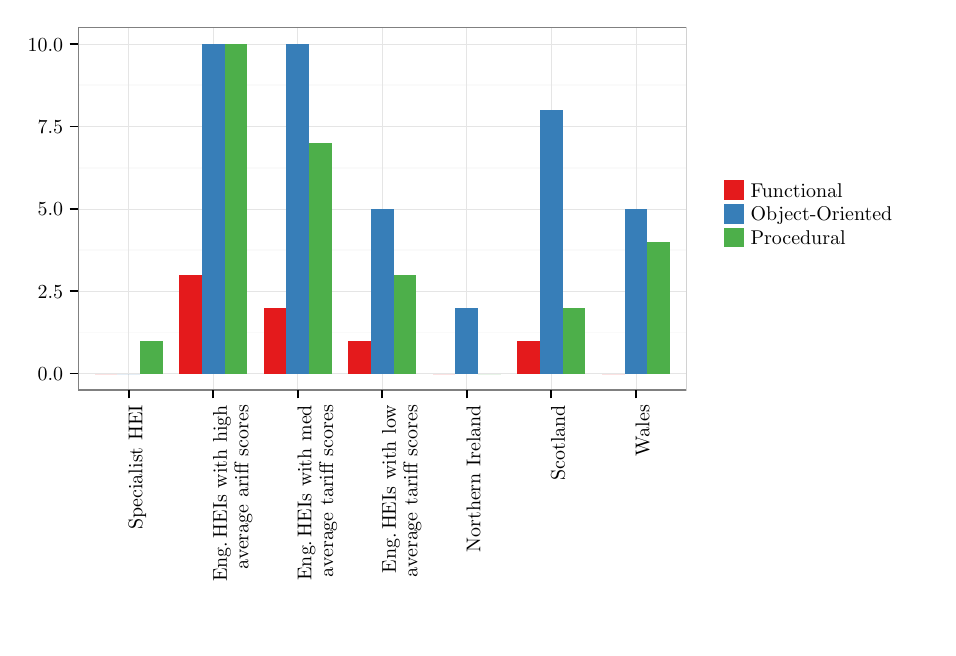
\begin{tikzpicture}[x=1pt,y=1pt]
\definecolor{fillColor}{RGB}{255,255,255}
\path[use as bounding box,fill=fillColor,fill opacity=0.00] (0,0) rectangle (325.21,216.81);
\begin{scope}
\path[clip] (  0.00,  0.00) rectangle (325.21,216.81);
\definecolor{drawColor}{RGB}{255,255,255}
\definecolor{fillColor}{RGB}{255,255,255}

\path[draw=drawColor,line width= 0.6pt,line join=round,line cap=round,fill=fillColor] (  0.00,  0.00) rectangle (325.21,216.81);
\end{scope}
\begin{scope}
\path[clip] ( 18.20, 85.85) rectangle (238.06,216.81);
\definecolor{fillColor}{RGB}{255,255,255}

\path[fill=fillColor] ( 18.20, 85.85) rectangle (238.06,216.81);
\definecolor{drawColor}{gray}{0.98}

\path[draw=drawColor,line width= 0.6pt,line join=round] ( 18.20,106.68) --
	(238.06,106.68);

\path[draw=drawColor,line width= 0.6pt,line join=round] ( 18.20,136.45) --
	(238.06,136.45);

\path[draw=drawColor,line width= 0.6pt,line join=round] ( 18.20,166.21) --
	(238.06,166.21);

\path[draw=drawColor,line width= 0.6pt,line join=round] ( 18.20,195.98) --
	(238.06,195.98);
\definecolor{drawColor}{gray}{0.90}

\path[draw=drawColor,line width= 0.2pt,line join=round] ( 18.20, 91.80) --
	(238.06, 91.80);

\path[draw=drawColor,line width= 0.2pt,line join=round] ( 18.20,121.57) --
	(238.06,121.57);

\path[draw=drawColor,line width= 0.2pt,line join=round] ( 18.20,151.33) --
	(238.06,151.33);

\path[draw=drawColor,line width= 0.2pt,line join=round] ( 18.20,181.09) --
	(238.06,181.09);

\path[draw=drawColor,line width= 0.2pt,line join=round] ( 18.20,210.86) --
	(238.06,210.86);

\path[draw=drawColor,line width= 0.2pt,line join=round] ( 36.52, 85.85) --
	( 36.52,216.81);

\path[draw=drawColor,line width= 0.2pt,line join=round] ( 67.05, 85.85) --
	( 67.05,216.81);

\path[draw=drawColor,line width= 0.2pt,line join=round] ( 97.59, 85.85) --
	( 97.59,216.81);

\path[draw=drawColor,line width= 0.2pt,line join=round] (128.13, 85.85) --
	(128.13,216.81);

\path[draw=drawColor,line width= 0.2pt,line join=round] (158.66, 85.85) --
	(158.66,216.81);

\path[draw=drawColor,line width= 0.2pt,line join=round] (189.20, 85.85) --
	(189.20,216.81);

\path[draw=drawColor,line width= 0.2pt,line join=round] (219.74, 85.85) --
	(219.74,216.81);
\definecolor{fillColor}{RGB}{228,26,28}

\path[fill=fillColor] ( 24.30, 91.80) rectangle ( 32.45, 91.80);
\definecolor{fillColor}{RGB}{55,126,184}

\path[fill=fillColor] ( 32.45, 91.80) rectangle ( 40.59, 91.80);
\definecolor{fillColor}{RGB}{77,175,74}

\path[fill=fillColor] ( 40.59, 91.80) rectangle ( 48.73,103.71);
\definecolor{fillColor}{RGB}{228,26,28}

\path[fill=fillColor] ( 54.84, 91.80) rectangle ( 62.98,127.52);
\definecolor{fillColor}{RGB}{55,126,184}

\path[fill=fillColor] ( 62.98, 91.80) rectangle ( 71.13,210.86);
\definecolor{fillColor}{RGB}{77,175,74}

\path[fill=fillColor] ( 71.13, 91.80) rectangle ( 79.27,210.86);
\definecolor{fillColor}{RGB}{228,26,28}

\path[fill=fillColor] ( 85.38, 91.80) rectangle ( 93.52,115.61);
\definecolor{fillColor}{RGB}{55,126,184}

\path[fill=fillColor] ( 93.52, 91.80) rectangle (101.66,210.86);
\definecolor{fillColor}{RGB}{77,175,74}

\path[fill=fillColor] (101.66, 91.80) rectangle (109.81,175.14);
\definecolor{fillColor}{RGB}{228,26,28}

\path[fill=fillColor] (115.91, 91.80) rectangle (124.06,103.71);
\definecolor{fillColor}{RGB}{55,126,184}

\path[fill=fillColor] (124.06, 91.80) rectangle (132.20,151.33);
\definecolor{fillColor}{RGB}{77,175,74}

\path[fill=fillColor] (132.20, 91.80) rectangle (140.34,127.52);
\definecolor{fillColor}{RGB}{228,26,28}

\path[fill=fillColor] (146.45, 91.80) rectangle (154.59, 91.80);
\definecolor{fillColor}{RGB}{55,126,184}

\path[fill=fillColor] (154.59, 91.80) rectangle (162.73,115.61);
\definecolor{fillColor}{RGB}{77,175,74}

\path[fill=fillColor] (162.73, 91.80) rectangle (170.88, 91.80);
\definecolor{fillColor}{RGB}{228,26,28}

\path[fill=fillColor] (176.99, 91.80) rectangle (185.13,103.71);
\definecolor{fillColor}{RGB}{55,126,184}

\path[fill=fillColor] (185.13, 91.80) rectangle (193.27,187.05);
\definecolor{fillColor}{RGB}{77,175,74}

\path[fill=fillColor] (193.27, 91.80) rectangle (201.41,115.61);
\definecolor{fillColor}{RGB}{228,26,28}

\path[fill=fillColor] (207.52, 91.80) rectangle (215.66, 91.80);
\definecolor{fillColor}{RGB}{55,126,184}

\path[fill=fillColor] (215.66, 91.80) rectangle (223.81,151.33);
\definecolor{fillColor}{RGB}{77,175,74}

\path[fill=fillColor] (223.81, 91.80) rectangle (231.95,139.42);
\definecolor{drawColor}{gray}{0.50}

\path[draw=drawColor,line width= 0.6pt,line join=round,line cap=round] ( 18.20, 85.85) rectangle (238.06,216.81);
\end{scope}
\begin{scope}
\path[clip] (  0.00,  0.00) rectangle (325.21,216.81);
\definecolor{drawColor}{RGB}{0,0,0}

\node[text=drawColor,anchor=base east,inner sep=0pt, outer sep=0pt, scale=  0.72] at ( 12.80, 89.32) {0.0};

\node[text=drawColor,anchor=base east,inner sep=0pt, outer sep=0pt, scale=  0.72] at ( 12.80,119.09) {2.5};

\node[text=drawColor,anchor=base east,inner sep=0pt, outer sep=0pt, scale=  0.72] at ( 12.80,148.85) {5.0};

\node[text=drawColor,anchor=base east,inner sep=0pt, outer sep=0pt, scale=  0.72] at ( 12.80,178.61) {7.5};

\node[text=drawColor,anchor=base east,inner sep=0pt, outer sep=0pt, scale=  0.72] at ( 12.80,208.38) {10.0};
\end{scope}
\begin{scope}
\path[clip] (  0.00,  0.00) rectangle (325.21,216.81);
\definecolor{drawColor}{RGB}{0,0,0}

\path[draw=drawColor,line width= 0.6pt,line join=round] ( 15.20, 91.80) --
	( 18.20, 91.80);

\path[draw=drawColor,line width= 0.6pt,line join=round] ( 15.20,121.57) --
	( 18.20,121.57);

\path[draw=drawColor,line width= 0.6pt,line join=round] ( 15.20,151.33) --
	( 18.20,151.33);

\path[draw=drawColor,line width= 0.6pt,line join=round] ( 15.20,181.09) --
	( 18.20,181.09);

\path[draw=drawColor,line width= 0.6pt,line join=round] ( 15.20,210.86) --
	( 18.20,210.86);
\end{scope}
\begin{scope}
\path[clip] (  0.00,  0.00) rectangle (325.21,216.81);
\definecolor{drawColor}{RGB}{0,0,0}

\path[draw=drawColor,line width= 0.6pt,line join=round] ( 36.52, 82.85) --
	( 36.52, 85.85);

\path[draw=drawColor,line width= 0.6pt,line join=round] ( 67.05, 82.85) --
	( 67.05, 85.85);

\path[draw=drawColor,line width= 0.6pt,line join=round] ( 97.59, 82.85) --
	( 97.59, 85.85);

\path[draw=drawColor,line width= 0.6pt,line join=round] (128.13, 82.85) --
	(128.13, 85.85);

\path[draw=drawColor,line width= 0.6pt,line join=round] (158.66, 82.85) --
	(158.66, 85.85);

\path[draw=drawColor,line width= 0.6pt,line join=round] (189.20, 82.85) --
	(189.20, 85.85);

\path[draw=drawColor,line width= 0.6pt,line join=round] (219.74, 82.85) --
	(219.74, 85.85);
\end{scope}
\begin{scope}
\path[clip] (  0.00,  0.00) rectangle (325.21,216.81);
\definecolor{drawColor}{RGB}{0,0,0}

\node[text=drawColor,rotate= 90.00,anchor=base east,inner sep=0pt, outer sep=0pt, scale=  0.72] at ( 41.48, 80.45) {Specialist HEI};

\node[text=drawColor,rotate= 90.00,anchor=base east,inner sep=0pt, outer sep=0pt, scale=  0.72] at ( 72.01, 80.45) {~Eng.\,HEIs with high};

\node[text=drawColor,rotate= 90.00,anchor=base east,inner sep=0pt, outer sep=0pt, scale=  0.72] at ( 79.79, 80.45) {average ariff scores};

\node[text=drawColor,rotate= 90.00,anchor=base east,inner sep=0pt, outer sep=0pt, scale=  0.72] at (102.55, 80.45) {~Eng.\,HEIs with med};

\node[text=drawColor,rotate= 90.00,anchor=base east,inner sep=0pt, outer sep=0pt, scale=  0.72] at (110.33, 80.45) {average tariff scores};

\node[text=drawColor,rotate= 90.00,anchor=base east,inner sep=0pt, outer sep=0pt, scale=  0.72] at (133.09, 80.45) {~Eng.\,HEIs with low};

\node[text=drawColor,rotate= 90.00,anchor=base east,inner sep=0pt, outer sep=0pt, scale=  0.72] at (140.86, 80.45) {average tariff scores};

\node[text=drawColor,rotate= 90.00,anchor=base east,inner sep=0pt, outer sep=0pt, scale=  0.72] at (163.62, 80.45) {Northern Ireland};

\node[text=drawColor,rotate= 90.00,anchor=base east,inner sep=0pt, outer sep=0pt, scale=  0.72] at (194.16, 80.45) {Scotland};

\node[text=drawColor,rotate= 90.00,anchor=base east,inner sep=0pt, outer sep=0pt, scale=  0.72] at (224.69, 80.45) {Wales};
\end{scope}
\begin{scope}
\path[clip] (  0.00,  0.00) rectangle (325.21,216.81);
\definecolor{fillColor}{RGB}{255,255,255}

\path[fill=fillColor] (246.59,132.45) rectangle (316.68,170.21);
\end{scope}
\begin{scope}
\path[clip] (  0.00,  0.00) rectangle (325.21,216.81);
\definecolor{fillColor}{RGB}{228,26,28}

\path[fill=fillColor] (251.57,154.50) rectangle (258.69,161.62);
\end{scope}
\begin{scope}
\path[clip] (  0.00,  0.00) rectangle (325.21,216.81);
\definecolor{fillColor}{RGB}{55,126,184}

\path[fill=fillColor] (251.57,145.97) rectangle (258.69,153.08);
\end{scope}
\begin{scope}
\path[clip] (  0.00,  0.00) rectangle (325.21,216.81);
\definecolor{fillColor}{RGB}{77,175,74}

\path[fill=fillColor] (251.57,137.43) rectangle (258.69,144.54);
\end{scope}
\begin{scope}
\path[clip] (  0.00,  0.00) rectangle (325.21,216.81);
\definecolor{drawColor}{RGB}{0,0,0}

\node[text=drawColor,anchor=base west,inner sep=0pt, outer sep=0pt, scale=  0.72] at (261.20,155.58) {Functional};
\end{scope}
\begin{scope}
\path[clip] (  0.00,  0.00) rectangle (325.21,216.81);
\definecolor{drawColor}{RGB}{0,0,0}

\node[text=drawColor,anchor=base west,inner sep=0pt, outer sep=0pt, scale=  0.72] at (261.20,147.04) {Object-Oriented};
\end{scope}
\begin{scope}
\path[clip] (  0.00,  0.00) rectangle (325.21,216.81);
\definecolor{drawColor}{RGB}{0,0,0}

\node[text=drawColor,anchor=base west,inner sep=0pt, outer sep=0pt, scale=  0.72] at (261.20,138.51) {Procedural};
\end{scope}
\end{tikzpicture}
